\documentclass{article}

% if you need to pass options to natbib, use, e.g.:
%     \PassOptionsToPackage{numbers, compress}{natbib}
% before loading neurips_2021

% ready for submission
% \usepackage{cvpr}
\usepackage{neurips_2021}
\usepackage{times}
\usepackage{epsfig}
\usepackage{graphicx}
\usepackage{amsmath}
\usepackage{amssymb}
\usepackage{listings}
\usepackage{float}
\usepackage{subfigure}

% to compile a preprint version, e.g., for submission to arXiv, add add the
% [preprint] option:
%     \usepackage[preprint]{neurips_2021}

% to compile a camera-ready version, add the [final] option, e.g.:
%     \usepackage[final]{neurips_2021}

% to avoid loading the natbib package, add option nonatbib:
%    \usepackage[nonatbib]{neurips_2021}

\usepackage[utf8]{inputenc} % allow utf-8 input
\usepackage[T1]{fontenc}    % use 8-bit T1 fonts
\usepackage{hyperref}       % hyperlinks
\usepackage{url}            % simple URL typesetting
\usepackage{booktabs}       % professional-quality tables
\usepackage{amsfonts}       % blackboard math symbols
\usepackage{nicefrac}       % compact symbols for 1/2, etc.
\usepackage{microtype}      % microtypography
\usepackage{xcolor}         % colors

\title{CS182: Introduction to Machine Learning: \\ Image Super Resolution}

% The \author macro works with any number of authors. There are two commands
% used to separate the names and addresses of multiple authors: \And and \AND.
%
% Using \And between authors leaves it to LaTeX to determine where to break the
% lines. Using \AND forces a line break at that point. So, if LaTeX puts 3 of 4
% authors names on the first line, and the last on the second line, try using
% \AND instead of \And before the third author name.

\author{
  Bi Chunhao\\
  \texttt{bichh@shanghaitech.edu.cn} \\
  % examples of more authors
  % \And
  % Coauthor \\
  % Affiliation \\
  % Address \\
  % \texttt{email} \\
  % \AND
  % Coauthor \\
  % Affiliation \\
  % Address \\
  % \texttt{email} \\
  % \And
  % Coauthor \\
  % Affiliation \\
  % Address \\
  % \texttt{email} \\
  % \And
  % Coauthor \\
  % Affiliation \\
  % Address \\
  % \texttt{email} \\
}

\begin{document}

\maketitle

%%%%%%%%% ABSTRACT
\begin{abstract}
  This is the final project of CS182, here we focused on a specific application called Image Super Resolution,
  which generates a higher resolution images based on the raw input. 
  We compared several existing algorithms and carried out some experiments to find the most suitable solution.
  \end{abstract}
  
  %%%%%%%%% BODY TEXT
  \section{Introduction}
  Super-resolution(SR) is a technology to restore a high-resolution(HR) image from a low-resolution(LR) one. 
  With the development of neural network, some new SR methods based on deep neural network achieve better performance than traditional algorithm. 
  These methods make the topic more and more popular. SR can be used in many areas, from commercial usage to daily entertainment. 
  For the former, image restoration is important in many fields including medical, military and communication. 
  Daily usage includes restoration of animations and meme images, and also photos.
  
  A typical field using this technology is remote sensing. 
  Remote sensing need to collect electromagnetic information to generate images, while the collection process is inevitably restricted by accuracy of current imaging sensors and complex atmospheric conditions. 
  Neural network based super-resolution technology, although not so mature for now, have potential to help solve these problems. 
  In our project, we will test and compare some cutting-edge network algorithms on super-resolution of images, including some specific tests on remote sensing images.
  
  In \cite{9}, author tested and compared learning-based, interpolation based, frequency domain based, 
  and probability based SR methods on remote sensing image reconstruction. And accept SR's usage in this field.
  
  There are specifically designed networks for upscaling remote sensing images. 
  An aerial image super-resolution method based on convolutional neural networks (CNNs) is mentioned in  \cite{10}.
  
  
  \section{Related Work}
  \subsection{CNN methods}
  Since the appearance of SRCNN \cite{6}, many achievements on combination of SR and neural network has been made by researchers. 
  As FSRCNN \cite{1} and ESPCN \cite{2}, which is based on CNNs, has simple structure and reasonable computation complexity. 
  LapSRN \cite{3} has multiple level CNNs structure. 
  EDSR \cite{4} are motivated by ResNet \cite{7}, which is proposed dealing with vanishing gradient problem caused when more layers are added to the network.
  Recent research direction is to extend depth of the network and the amount of training sets to achieve better SR performance.
  However, with the model being deeper and deeper, the time cost also increases.
  
  \subsection{GAN}
  A scenario for SR is the loss of detailed information. 
  Without appending more information to the raw image, the model can hardly create a realistic SR result.
  Due to the little information carried by the LR image, the restored image will meet a limitation.
  This is where GAN is taken into consideration.
  
  GAN(Generative Adversarial Networks) based SR is proposed recently. 
  It means to generate details that are not provided by the origin image, and the details must be credible and consistent to origin image structure.
  For example, Real-ESRGAN \cite{5}, an expansion on real photos from ESRGAN, can extend an animation image or a landscape photo into a higher-resolution one with smooth outline and good look.
  GAN usually can generate images with a fantastic perceived feeling, but sometimes the result will even feel unrealistic due to the details appended.
  
  \begin{figure}[H]
      \centering
      \subfigure[LR]{
      \begin{minipage}[t]{0.45\linewidth}
      \centering
      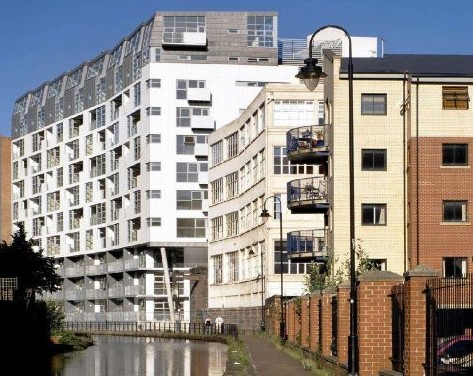
\includegraphics[width=1.2in]{images/building.jpg}
      \end{minipage}
      }
      \subfigure[Real-ESRGAN]{
      \begin{minipage}[t]{0.45\linewidth}
      \centering
      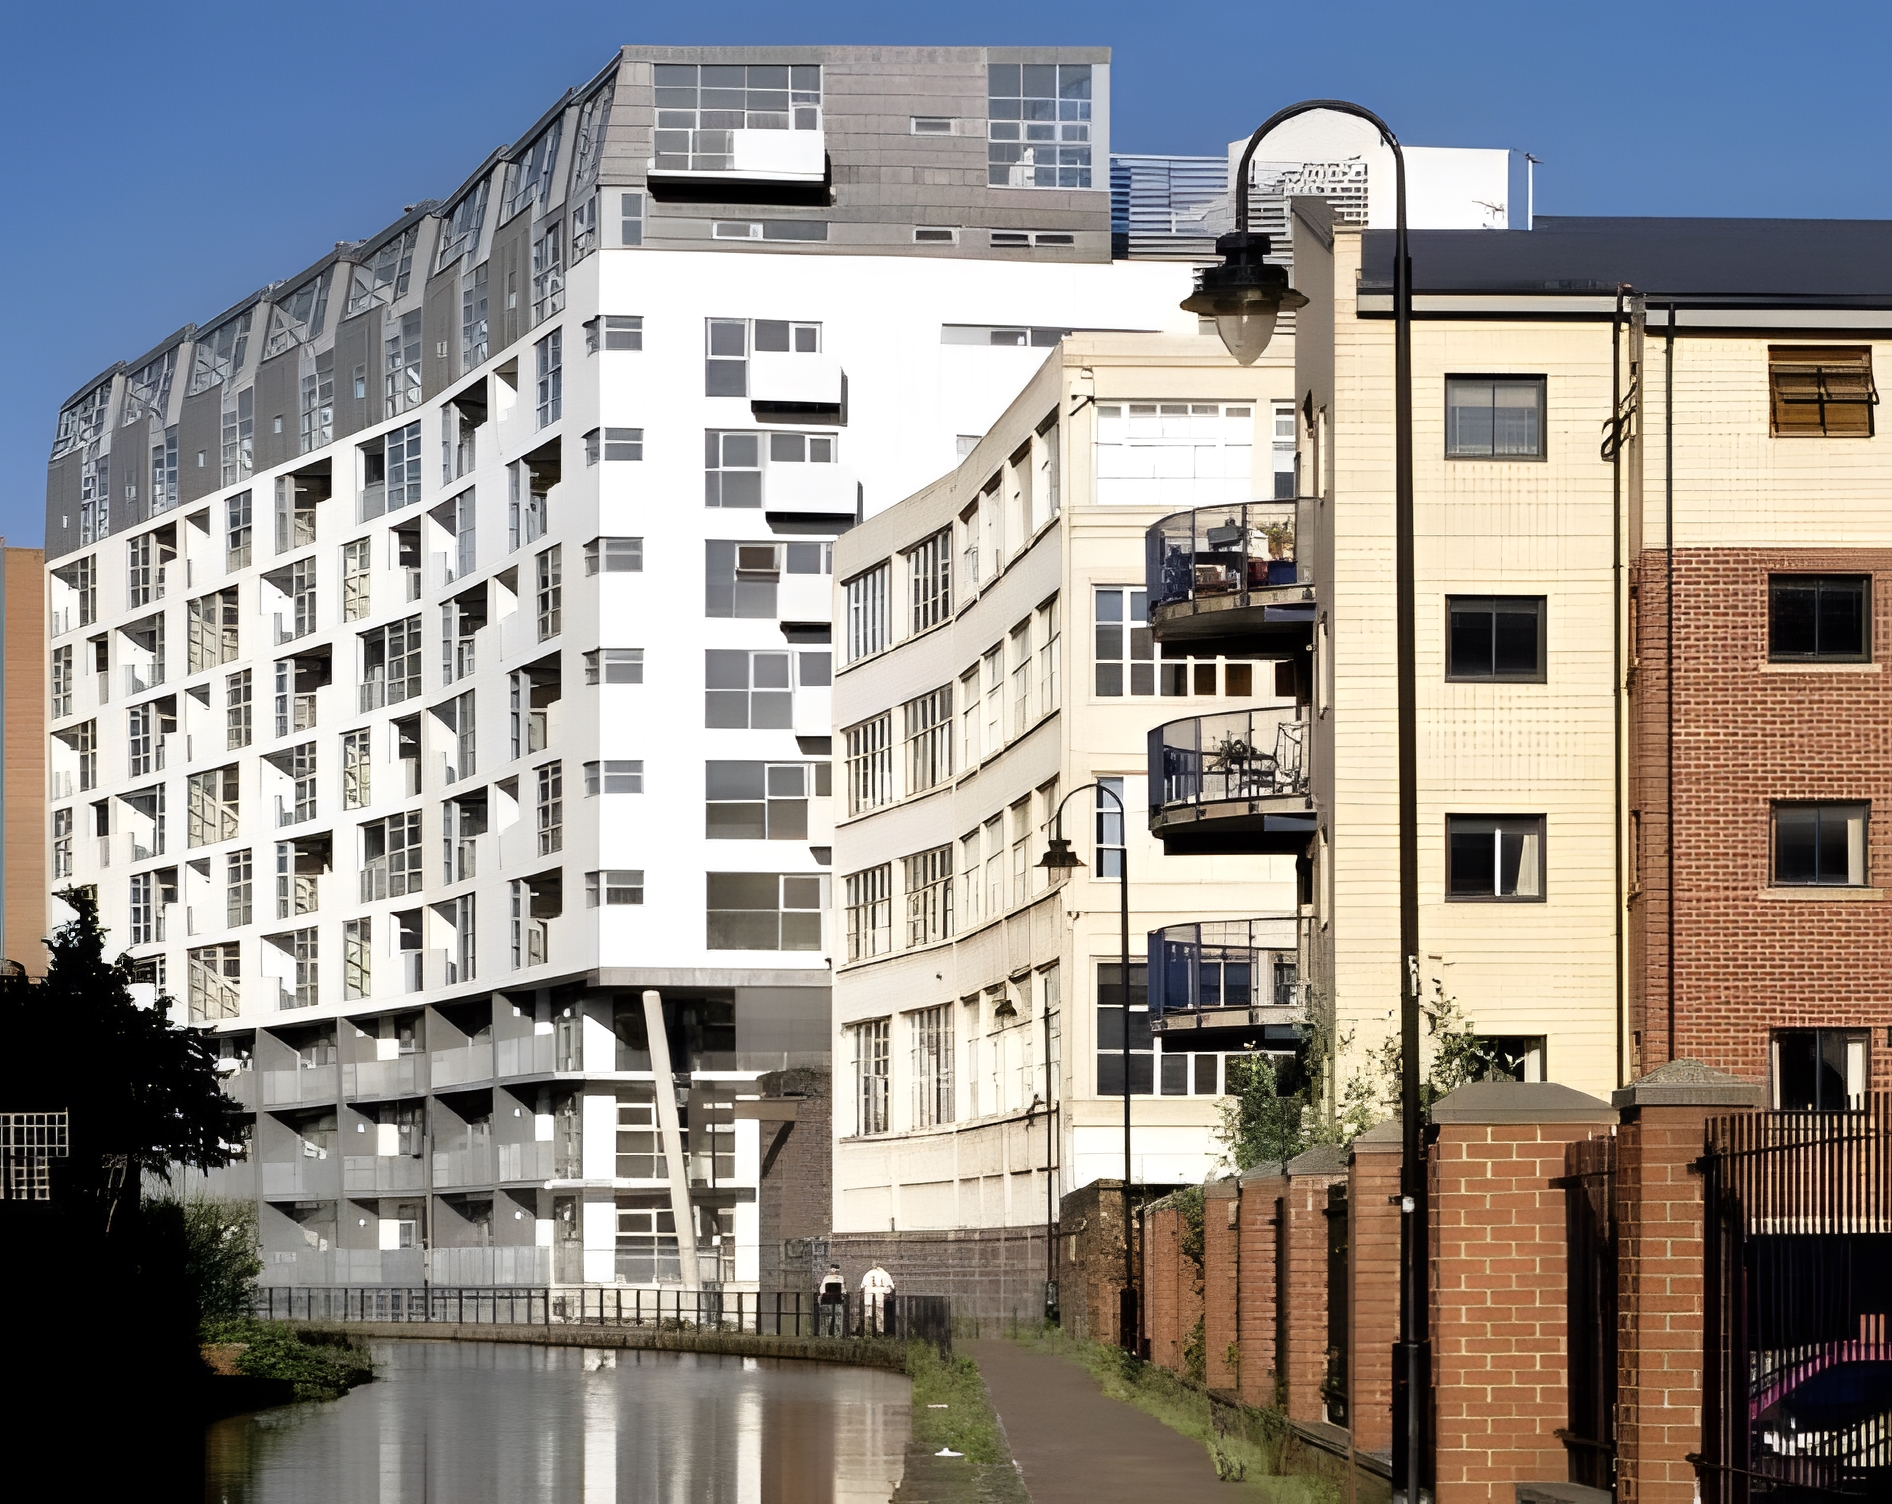
\includegraphics[width=1.2in]{images/building_out.jpg}
      \end{minipage}
      }
      \caption{Detailed generated HR image}
  \end{figure}
  As the details are not equally important in every using field of SR, GAN are not taken into comparison in this project.
  
  
  
  
  \section{Different solutions} 
  \subsection{Bicubic}
  Bicubic is an interpolation method. For each pixel in the new image, 16 raw pixels around will be taken into consideration.
  The difference between this method and Bilinear interpolation is that it takes two cubic function on the two direction.
  Experiments showed that Bicubic can restore more accurately than Bilinear, with little more time spent.
  Another method called Nearest Neighbor, which as it is saying, select values from the nearest pixel, runs the most fast.
  For some commercial image editing software products, the method is used for its fast speed. However, this method may result in a serious aliased defect.
  
  In this project, Bicubic method is used to compare with other methods.
  It may be the slowest in the three mentioned, but still is much faster compared to the methods using CNN.
  
  \subsection{FSRCNN}
  FSRCNN \cite{1} is also called fast-SRCNN. 
  It is designed by Chao Dong, Chen Change Loy, and Xiaoou Tang, 
  who first put forward applying deep learning neural network to super-resolution. 
  \begin{figure}[H]
      \centering
      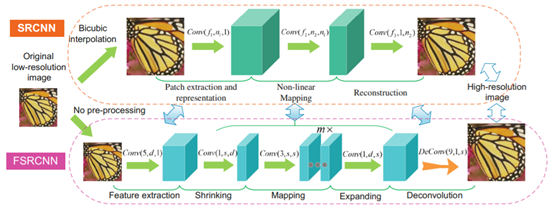
\includegraphics[scale = 0.4]{images/FSRCNN.png}
      \caption{The network structure of SRCNN and FSRCNN}
  \end{figure}
  Fast-SRCNN accelerating the current SRCNN \cite{6}. 
  SRCNN upscales LR image to target size by bicubic interpolation before actually entering the network. 
  While FSRCNN just take LR images as the input, and conducts upsampling by the deconvolution layer at the end of the net work. 
  This change leads to 2 main difference: 
  \begin{itemize}
      \item Directly, no need to cost time carrying out Bicubic operation.
      \item Conv operation on LR image is less costly.
  \end{itemize}
  With less computational complexity, FSRCNN can support a deeper network and achieve a better effect.
  FSRCNN takes LR images as the input and carry out feature extraction. 
  Then, replacing the non-linear mapping step, FSRCNN takes shrinking, mapping and expanding steps instead. 
  And finally construct the desired HR image with a deconvolution operation. 
  FSRCNN take PReLU as the activation function and L2 as loss.
  
  \subsection{ESPCN}
  ESPCN \cite{2} is also motivated by SRCNN. Like FSRCNN, ESPCN takes LR images as the input and have low computational complexity. 
  \begin{figure}[H]
      \centering
      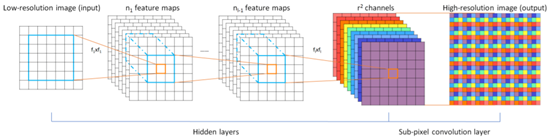
\includegraphics[scale = 0.4]{images/ESPCN.png}
      \caption{The network structure of ESPCN}
  \end{figure}
  The author team implement a more efficient sub-pixel convolution layer for learn. 
  ESPCN takes an LR image as the input. 
  For a network with L layers, ESPCN will learn L-1 upscaling filters for every channel, and finally a deconvolution layer that recovering resolution of the image. 
  The use of deconvolution layer had shown good effect in other in visual field and cause low cost, that's why both FSRCNN and ESPCN choose to use deconvolution layer. 
  And operation also enable cheaper convolution operations to be used in hidden layers.
  ESPCN take $tanh()$ as activation function and L2 as loss.
  
  \subsection{LapSRN}
  LapSRN's full name is Laplacian Pyramid Super-Resolution Network \cite{3}. 
  In comparison with previous 2 models, LapSRN has deeper network structure, and has many properties. 
  \begin{figure}[H]
      \centering
      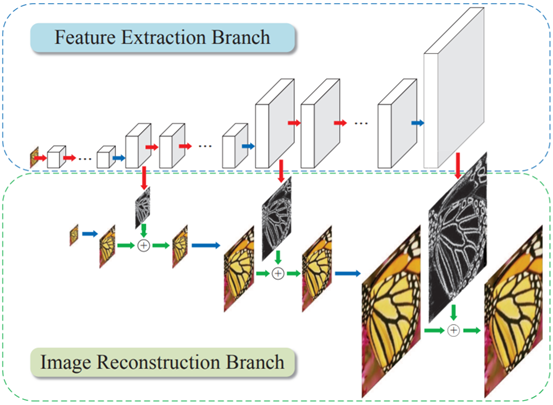
\includegraphics[scale = 0.4]{images/LapSRN.png}
      \caption{The network structure of LapSRN}
  \end{figure} 
  
  Despite the detailed network implementation, LapSRN have 3 main characteristic.
  \begin{itemize}
      \item LapSRN has multiple-level structure, every structure can conduct a 2x upscaling on input image and output of previous level can be taken as input of next level. 
      As a result, LapSRN can support up to 8x upscaling, while most model only support 4x. 
      \item In each level, feature extraction conduct first, then upscaling by a deconvolution layer to 2x size. 
      LapSRN also motivated by Residual Learning \cite{7}, the upsampled image is then combined (using element-wise summation) with the predicted residual image from the feature extraction branch to produce a high-resolution output image.
      \item The author team think L2 loss is not good enough for SR learning and is inevitably to generate blurry predictions. 
      So, LapSRN choose another loss: Charbonnier penalty function (a differentiable variant of L1 norm) \cite{3}. 
      This loss is considered at the end of every level.
  \end{itemize}
  
  \subsection{EDSR}
  The design of EDSR is based on the SRResNet \cite{8}, which is motivated by ResNet \cite{7} and achieve good performance in solving time/memory issue in SR. 
  What's more, EDSR has won NTIRE2017 SR Challenge.
  \begin{figure}[H]
      \centering
      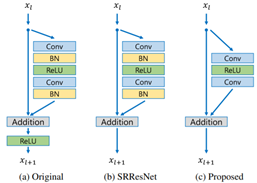
\includegraphics[scale = 0.6]{images/EDSR1.png}
      \caption{Comparison of residual blocks in ResNet, SRResNet and EDSR}
  \end{figure} 
  \begin{figure}[H]
      \centering
      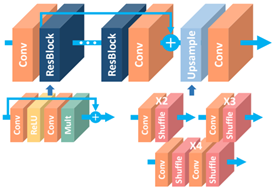
\includegraphics[scale = 0.6]{images/EDSR2.png}
      \caption{The architecture of the proposed single-scale SR network (EDSR)}
  \end{figure} 
  the author team find the batch normalization layers get rid of range flexibility from networks by normalizing the features. 
  Since SR is low-level computer visual problem. These BN block in original ResNet may not do good for SR. 
  So, EDSR remove these BN layers is better, which further lead to approximately 40\% of memory usage saving. \cite{4}
  EDSR use L1 loss instead of L2, because author team find L1 loss provides better convergence.
  
  
  
  \section{Results and Experiments}
  \subsection{Testing}
  \subsubsection*{Models}
  Due to time and equipments limitations, we can't train all the models by ourselves, so
  we take the $\times 4$ version trained models of 
  \href{https://github.com/Saafke/EDSR_Tensorflow/tree/master/models}{EDSR},
  \href{https://github.com/Saafke/FSRCNN_Tensorflow/tree/master/models}{FSRCNN},
  \href{https://github.com/fannymonori/TF-ESPCN/tree/master/export}{ESPCN},
  \href{https://github.com/fannymonori/TF-LapSRN/tree/master/export}{LapSRN} from GitLab.
  Real-ESRGAN's model doesn't join the following experiment. 
  Team of Real-ESRGAN provide their own executable file with hardware acceleration, convenient but can't match our requirement.
  
  \subsubsection*{Evaluation Metrics}
  \begin{itemize}
      \item PSNR 
      
      PSNR (Peak Signal to Noise Ratio) is a generally used measuring method for image resolution.
      PSNR is the ratio of maximum signal power and the average power.
      The definition is:
      \begin{align*}
          PSNR = 10log_{10}\frac{MaxValue^2}{MSE} = 10log_{10}\frac{255}{MSE}
      \end{align*}
      Where MSE(Mean Squared Error) denotes the average power between the groundtruth and the result image.
  
      However, PSNR scores is not consistent to the quality human eye perceives, sometimes a higher PSNR score image may look worse.
      The reason is that human eye is not sensitive to high frequency noise, which is usually separately distributed. 
      The perception is influenced by the whole surrounding area in a low frequency way.
      Below is some images with same PSNR scores, but is quite different for human perception. 
      \begin{figure}[H]
          \centering
          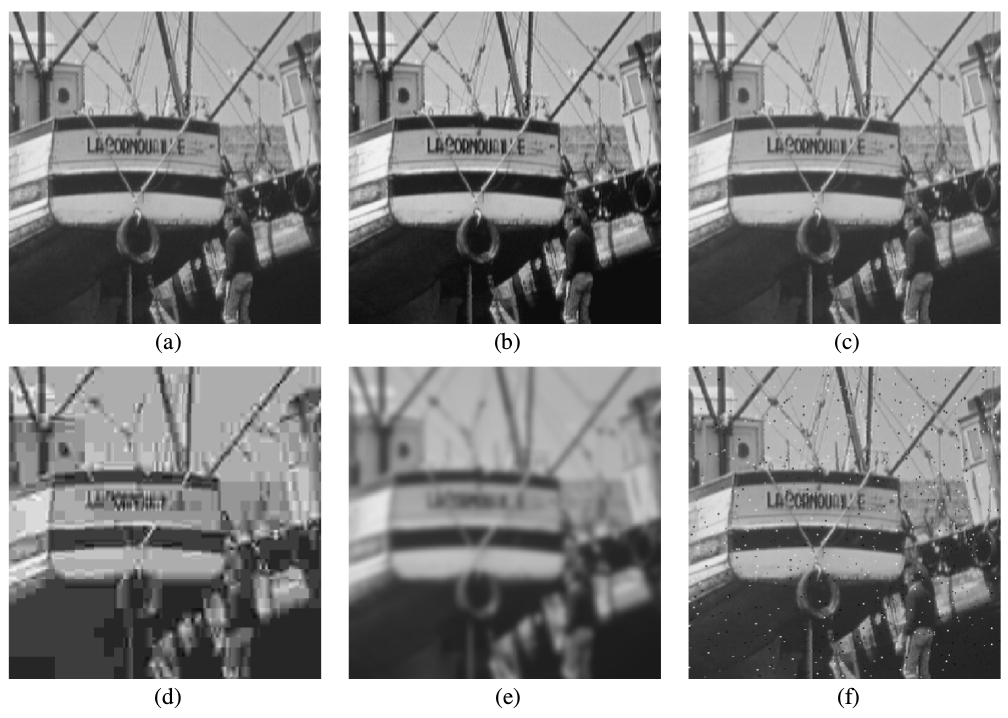
\includegraphics[scale = 0.3]{images/PSNR.png}
          \caption{Same PSNR scores with different distortions}
      \end{figure}
  
      \item SSIM
      
      SSIM (Structural Similarity Index) is a method to evaluate the similarity of two images.
      It is based on the whole structure, with less focus on pixelwise error. 
      SSIM contains three evaluation aspects:
      \begin{itemize}
          \item Luminance
          \item Contrast
          \item Structure
      \end{itemize}
      The detailed calculation is complicated. A general pipeline is as follows:
      \begin{figure}[H]
          \centering
          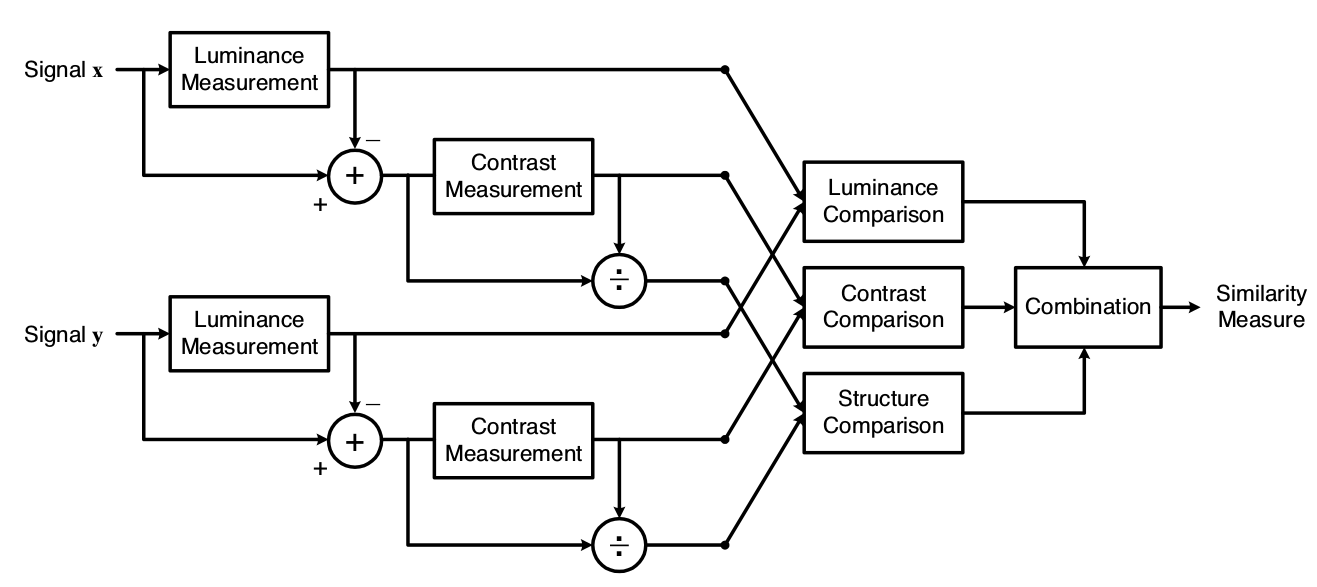
\includegraphics[scale = 0.2]{images/SSIM.png}
          \caption{Same PSNR scores with different distortions}
      \end{figure}
      The Luminance can be represented as mean value, the Contrast as variance after normalization, 
      and the structure as coefficient of association (fraction of covariance and variance products).
  
  \end{itemize}
  
  
  \subsection{Results}
  The testing set we take is DIV2K High Resolution dataset \href{https://data.vision.ee.ethz.ch/cvl/DIV2K}{DIV2K\_valid\_HR} 
  which contains 100 2K images, and negative-image-set in \href{https://hyper.ai/datasets/5422}{NWPU VHR-10} which contains 1K images taken from remote sensors.
  The former is a mixture set of varieties of objects, so we considered it as a general case.
  NWPU VHR-10 data set is a challenging ten-class geospatial object detection data set, images of which are mostly come from remote sensing equipments. 
  For this, we randomly selected an area of size $256\times 256$ for each image to test.
  We first downsample the images to 1/4 size, and then use the model to generate images with origin resolution.
  The evaluation result is calculated with the groundtruth image.
  The average scores are as follows:
  \begin{table}[H]
      \centering
      \caption{Image Evaluation on DIV2K}
      \begin{tabular}{|l|l|l|l|}
      \hline
      Average Evaluation  & PSNR   & SSIM   & Time spent  \\ \hline
      Bicubic             & 26.228 & 0.7722 & 0.0025      \\ \hline
      EDSR                & 27.789 & 0.8091 & 34.844      \\ \hline
      ESPCN               & 26.689 & 0.7737 & 0.0840      \\ \hline
      FSRCNN              & 26.580 & 0.7704 & 0.1302      \\ \hline
      LapSRN              & 26.710 & 0.7741 & 2.9266      \\ \hline
      \end{tabular}
  \end{table}
  \begin{table}[H]
      \centering
      \caption{Image Evaluation on NWPU VHR-10}
      \begin{tabular}{|l|l|l|l|}
      \hline
      Average Evaluation  & PSNR   & SSIM   & Time spent  \\ \hline
      Bicubic             & 28.679 & 0.7591 & 0.0003      \\ \hline
      EDSR                & 30.090 & 0.7972 & 1.0144      \\ \hline
      ESPCN               & 28.882 & 0.7589 & 0.0040      \\ \hline
      FSRCNN              & 28.647 & 0.7556 & 0.0038      \\ \hline
      LapSRN              & 28.915 & 0.7589 & 0.0739      \\ \hline
      \end{tabular}
  \end{table}
  To be noticed, EDSR results in a great accuracy. 
  However, due to the great size of its network, it also spent a lot of time than the others.
  
  
  \subsection{Visualization}
  If the scores are not familiar, some visual results can bring a more intuitive understanding.
  \begin{figure}[H]
      \centering
      \subfigure[Groundtruth]{
      \begin{minipage}[t]{0.3\linewidth}
      \centering
      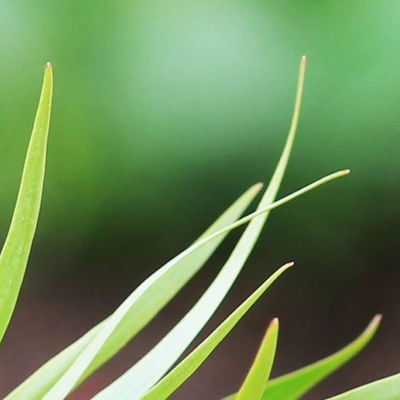
\includegraphics[width=1in]{images/plant_origin.png}
      \end{minipage}
      }
      \subfigure[Bicubic]{
      \begin{minipage}[t]{0.3\linewidth}
      \centering
      
\includegraphics[width=1in]{images/plant_bicubic.png}
      \end{minipage}
      }
      \subfigure[EDSR]{
      \begin{minipage}[t]{0.3\linewidth}
      \centering
      
\includegraphics[width=1in]{images/plant_EDSR.png}
      \end{minipage}
      }
  
      \subfigure[ESPCN]{
      \begin{minipage}[t]{0.3\linewidth}
      \centering
      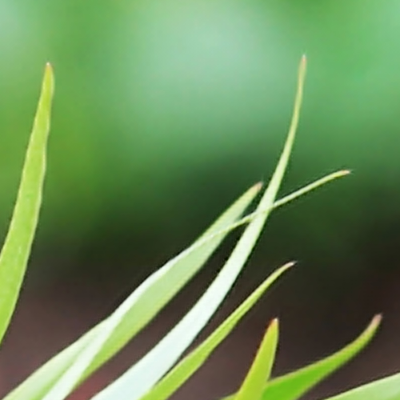
\includegraphics[width=1in]{images/plant_ESPCN.png}
      \end{minipage}
      }
      \subfigure[FSRCNN]{
      \begin{minipage}[t]{0.3\linewidth}
      \centering
      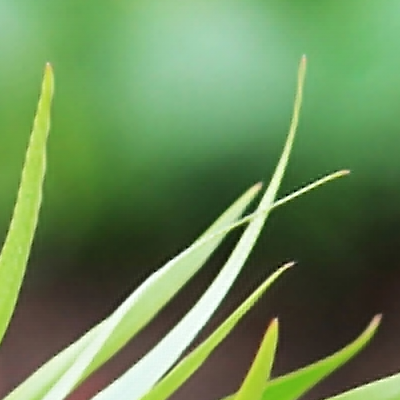
\includegraphics[width=1in]{images/plant_FSRCNN.png}
      \end{minipage}
      }
      \subfigure[LapSRN]{
      \begin{minipage}[t]{0.3\linewidth}
      \centering
      
\includegraphics[width=1in]{images/plant_LapSRN.png}
      \end{minipage}
      }
      \caption{Remote sensing pictures restoration}
  \end{figure}
  From the result above, we can tell that the model is useful for dealing with aliasing.
  Aliasing is a normal consequence when pictures are compressed into a lower resolution.
  The bicubic interpolation can't do well with this situation, 
  but the rest four methods can smoothen the images to be more realistic.
  
  As for remote sensing image restoration.
  We tested the models on such dataset. 
  Some visual results are shown here:
  \begin{figure}[H]
      \centering
      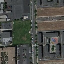
\includegraphics[width=1in]{images/rs_LR.png}
      \caption{Low resolution image}
  \end{figure}
  The LR image is generated from a HR one using nearest Neighbor method in opencv.
  Then the image is considered as the input in the testing algorithms.
  The result after the models are:
  \begin{figure}[H]
      \centering
      \subfigure[Groundtruth]{
      \begin{minipage}[t]{0.3\linewidth}
      \centering
      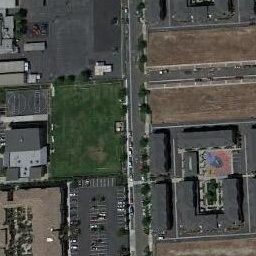
\includegraphics[width=1in]{images/rs_origin.png}
      \end{minipage}
      }
      \subfigure[Bicubic]{
      \begin{minipage}[t]{0.3\linewidth}
      \centering
      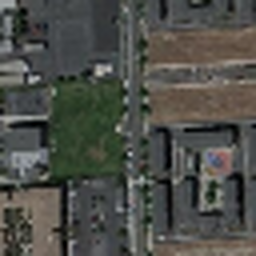
\includegraphics[width=1in]{images/rs_bicubic.png}
      \end{minipage}
      }
      \subfigure[EDSR]{
      \begin{minipage}[t]{0.3\linewidth}
      \centering
      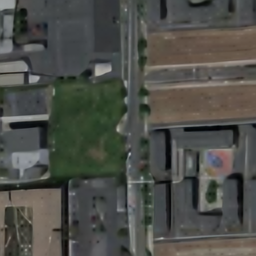
\includegraphics[width=1in]{images/rs_EDSR.png}
      \end{minipage}
      }
  
      \subfigure[ESPCN]{
      \begin{minipage}[t]{0.3\linewidth}
      \centering
      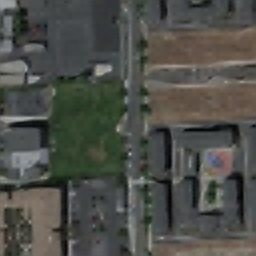
\includegraphics[width=1in]{images/rs_ESPCN.png}
      \end{minipage}
      }
      \subfigure[FSRCNN]{
      \begin{minipage}[t]{0.3\linewidth}
      \centering
      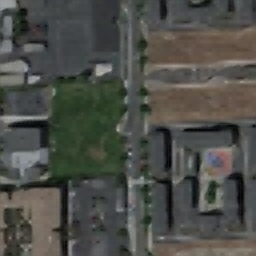
\includegraphics[width=1in]{images/rs_FSRCNN.png}
      \end{minipage}
      }
      \subfigure[LapSRN]{
      \begin{minipage}[t]{0.3\linewidth}
      \centering
      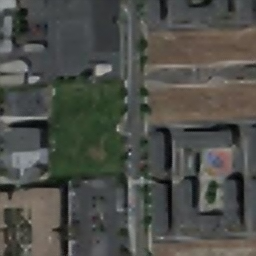
\includegraphics[width=1in]{images/rs_LapSRN.png}
      \end{minipage}
      }
      \caption{Restoration from aliased compression}
  \end{figure}
  We can tell that there are great differences between the raw image and the restored ones.
  Also, different algorithms carried out difference results, but generally the CNN ones tend to smoothen the image.
  The smoothened images have more clear edge representations and are easier to distinguish building.
  Some high frequency details are omitted, which are not important. The low frequency components are kept in the results.
  
  \section{Conclusion}
  
%   {\small
%   \bibliographystyle{ieee_fullname}
%   \bibliography{reportbib}
%   }
  

\end{document}
